
% !TEX root = ../../phdthesis_tawatr.tex 
\renewcommand{\thisdir}{_content/gamma}
\renewcommand{\figdir}{\thisdir/_fig}
\section{Local and regional distortion indicators}

%% ==== Introductory paragraph
This section shows the example of local and regional distortion indicators (Eqs \ref{eq:gamma_local_def} and \ref{eq:gamma_regional_def}) derived from the synthetic 1D and 3D examples in Sections \ref{sect:example_1d} and \ref{sect:example_3d}, respectively.

%% ==== local 1D
%\begin{itemize}

%	\item 
	In this test, these local distortion indicators are obtained by applying Eq. \eqref{eq:gamma_local_def} to the det and ssq impedances from the 1D dataset distorted with the distortion parameter with an SD of 0.3 (as shown in Figure \ref{fig:resp1d_individual_all_distorted_sd3a}), for example.
%	\item 
	As shown earlier, the local distortion indicators derived from distorted 1D data are shifted upward (greater than unity) and remain real-valued.
%	\item 
	The local distortion indicators are shifted irregularly depending on the strength of shear and splitting parameters at individual sites (Figure \ref{fig:gamma_local_example_1d}). 
%	\item 
	In addition, the calculated local distortion indicator from the data distorted with $\gtes = (1.20,0.11,-0.37,0.49)$, for example, agrees well with the actual value (gray circles and dashed line in Figure \ref{fig:gamma_local_example_1d}, respectively).
	Note that the actual local distortion indicator is calculated by substituting the shear and splitting parameters of $-0.37$ and 0.49 into Eq. \eqref{eq:gamma_1d_analytic}.
%\end{itemize}

%% ==== local 3D
%\begin{itemize}
%	\item 
	For 3D cases, the local distortion indicators contain both the frequency dependent and independent features (Eq. \ref{eq:gamma_approx}). The frequency independent part is mainly due to the shear and splitting parameters, which are real-valued, while the frequency dependent part is ascribed by the difference between the ssq and det impedances at individual sites, which is complex-valued and rather weak in general.
%	\item 
	As with the 1D example, the example of local distortion indicators from distorted 3D data (Figure \ref{fig:gamma_regional_example_3d}) are also obtained by applying Eq. \eqref{eq:gamma_local_def} to the 3D data distorted with the distortion parameter with an SD of 0.3 (as shown in Figure \ref{fig:resp3d_individual_all_distorted_sd3a}).
	In contrast to the 1D case, the local distortion indicators from distorted 3D data show a frequency-dependent feature and become complex-valued, which depends on how strong the inductive effect from the underlying structure is and the galvanic distortion strength posed in the data. 
%	\item
	The local distortion indicator derived from the data at the station \texttt{syn08}, which is distorted by $\gtes$ of $(1.20,0.11,-0.37,0.49)$, are compared with the actual value of the local distortion indicators.
	Although the local distortion indicator is deviated because of the inductive effect of the underlying structure, it still oscillates about the actual values (gray circles and dashed line in Figure \ref{fig:gamma_local_example_3d}). Hence the local distortion indicator can be used to indicate the strength of shear and splitting effects.
%\end{itemize}

%% ==== Gamma local
\begin{figure}[t]
	\centering
	\subfigure[]{
		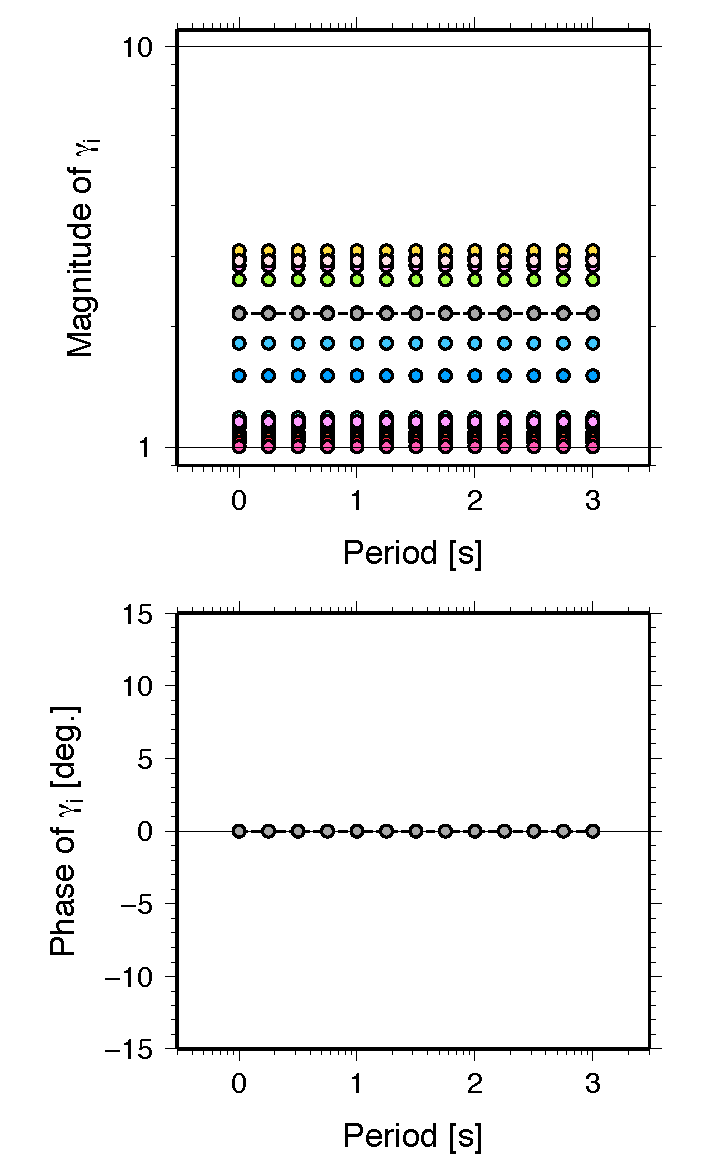
\includegraphics[scale=\plotmtrespscale]{\figdir/lyr11a_n25_d13a_distorted-sd3a-gtes_gamma_magphs_merged.pdf}
		\label{fig:gamma_local_example_1d}
	}
	\subfigure[]{
		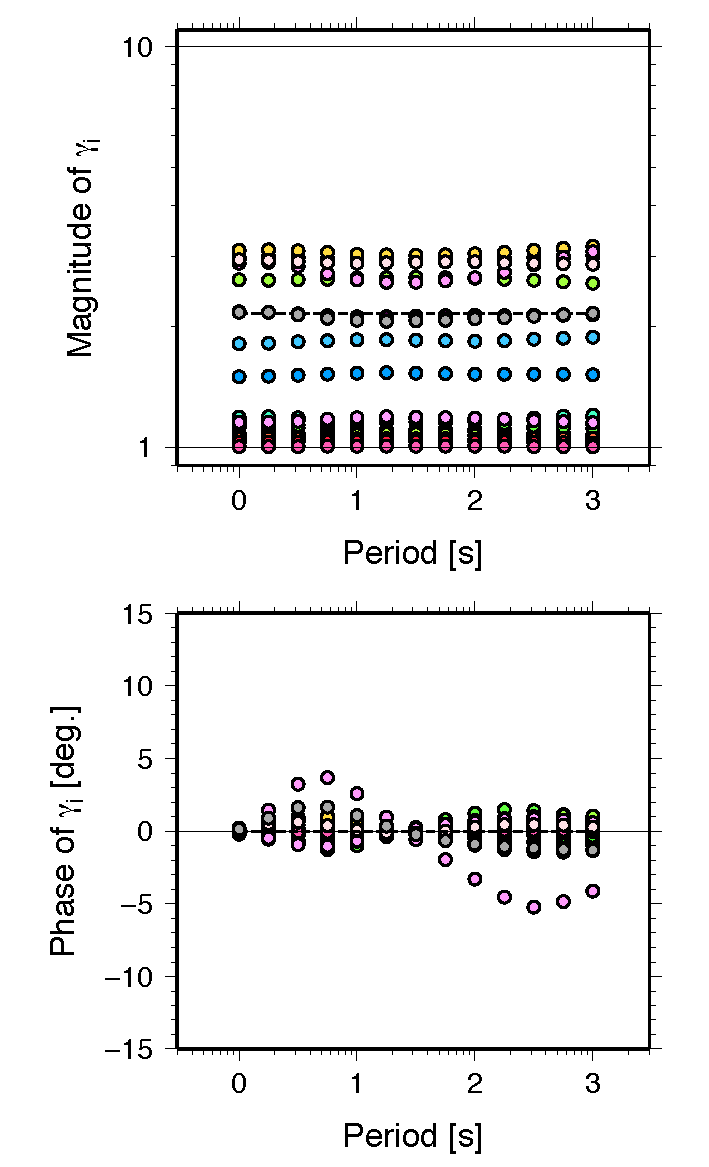
\includegraphics[scale=\plotmtrespscale]{\figdir/m02a-lyr11a_cb12-h0a2a-d05a-t01a_dr-e43n42_cb1X_loc-regi0_c-s40k-p0p0-pp1_d13a_distorted-sd3a-gtes_gamma_magphs_merged.pdf}
		\label{fig:gamma_local_example_3d}
	}
	\caption[Local distortion indicators from 1D and 3D data]{Local distortion indicators from the distorted (a) 1D and (b) 3D data (in Sections \ref{sect:example_1d} and \ref{sect:example_3d}, respectively) where a set of distortion parameters with an SD of 0.3 was applied. Examples of 1D and 3D data at station \texttt{syn08} distorted with $(g, t, e, s) = (1.20, 0.11, -0.37, 0.49)$ (gray circles) are compared with the actual values of the local distortion indicator at this station (dashed lines)}
	\label{fig:gamma_local_example}
\end{figure}

%%%% ==== Local exception
However, if the strong 3D effect (e.g., coastal effect) or the inductive distortion is contained, the local distortion indicator would become very frequency dependent and rather complex valued. In such a case, the treatment of distortion as galvanic orgin is not allowed. In other words, the local distortion indicator is able to indicate the period range where the data is inductively distorted as well as galvanically distorted. Thus the local distortion indicator will help judge the validity of applying phase tensor, because the phase tensor is defined for the case with the galvanic distortion only.





%%% ==== Local distortion indicator: Mean
The mean local distortion indicators $\gammaimean$ of the 1D and 3D dataset distorted with the set of distortion parameters with SD of 0.3 (Figures \ref{fig:gamma_1d_site} and \ref{fig:gamma_3d_site}) are calculated using Eq. \eqref{eq:gamma_local_mean_def}.
%
Compared to the local distortion indicators (Figures \ref{fig:gamma_local_example_1d} and \ref{fig:gamma_local_example_3d}), it is more convenient to identify the site-to-site strength of the shear and splitting effect.
%
They are shown in comparison with the actual local distortion indicators $\gammai$, which are calculated by substituting the synthetic shear and splitting parameters at each station into Eq. \eqref{eq:gamma_local_def}.
%
We also define the percentage difference between the mean local distortion indicator and the actual local distortion indicators for validation purposes:
	\begin{equation}
		\mathcal{P}(\gammaimean) = \frac{\gammaimean - \gammai}{\gammai} \times 100\%.
	\end{equation}	
In the 1D case, the mean local distortion indicator is able to correctly estimate the strength of galvanic distortion with zero difference (Figure \ref{fig:gamma_1d_site}).
%
As shown earlier, the underlying structure may affect the local distortion indicator in 3D case as a frequency dependent contribution.
%
Here, the error bar is set to the standard deviation in order to represent the dispersion of the frequency dependent part in the local distortion indicator. For example, the station \texttt{syn02} has the significant frequency-dependent variation.
Although some errors in estimating the galvanic distortion strength appear in the distorted 3D data (Figure \ref{fig:gamma_3d_site}), they are still in the acceptable range.

%% ==== The percentage difference of local distortion indicators 1-D
%\missingfigure[figwidth=6cm]{P. diff of local distortion indicators}
\begin{figure}[!t]
	\centering
	\subfigure[]{
		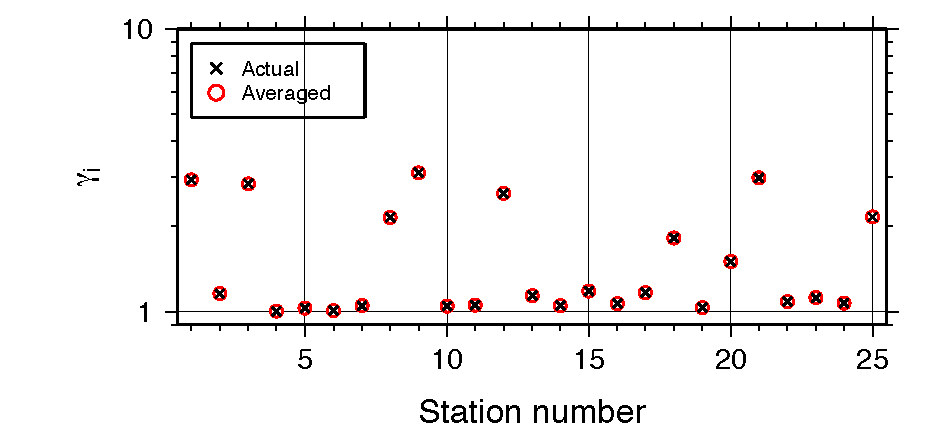
\includegraphics[scale=\plotdindmeanscale]{\figdir/lyr11a_n25_d13a_distorted-sd3a-gtes_gamma_est.pdf}
		\label{fig:gamma_1d_site_estimated}
	}
	\subfigure[]{
		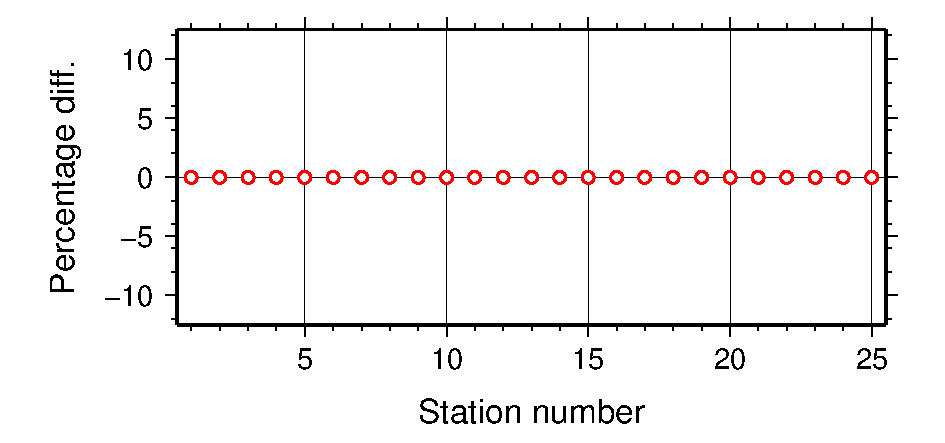
\includegraphics[scale=\plotdindmeanscale]{\figdir/lyr11a_n25_d13a_distorted-sd3a-gtes_gammapdiff.pdf}
		\label{fig:gamma_1d_site_pdiff}
	}
	\caption[Comparison of the actual and the mean local distortion indicators and percentage difference]{(a) Comparison of actual local distortion indicators (crosses) with the mean local distortion indicators (red circles) from the 1D example, where a set of distortion parameters with an SD of 0.3 was applied (Figure \ref{fig:resp1d_individual_all_distorted_sd3a}). (b) Percentage difference between the mean local distortion indicators and the actual ones.}
	\label{fig:gamma_1d_site}
\end{figure}
%% ==== The percentage difference of local distortion indicators 3-D
\begin{figure}[t]
	\centering
	\subfigure[]{
		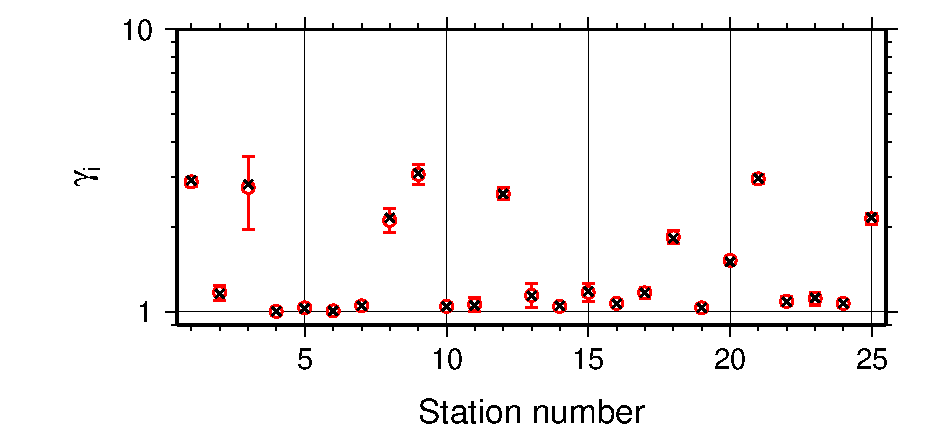
\includegraphics[scale=\plotdindmeanscale]{\figdir/m02a-lyr11a_cb12-h0a2a-d05a-t01a_dr-e43n42_cb1X_loc-regi0_c-s40k-p0p0-pp1_d13a_distorted-sd3a-gtes_gamma_est_esd}
		\label{fig:gamma_3d_site_estimated}
	}
	\subfigure[]{
		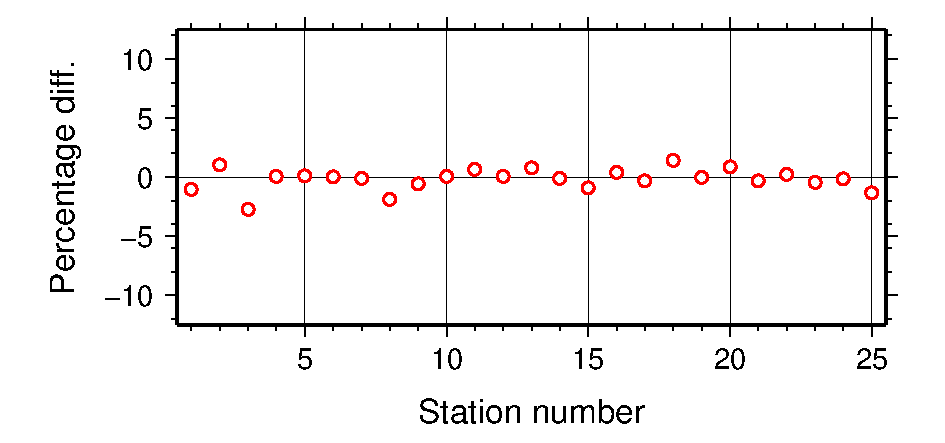
\includegraphics[scale=\plotdindmeanscale]{\figdir/m02a-lyr11a_cb12-h0a2a-d05a-t01a_dr-e43n42_cb1X_loc-regi0_c-s40k-p0p0-pp1_d13a_distorted-sd3a-gtes_gammapdiff_esd.pdf}
		\label{fig:gamma_3d_site_pdiff}
	}
	\caption{Same as Figure \ref{fig:gamma_1d_site} for the 3D example}
	\label{fig:gamma_3d_site}
\end{figure}


%% ==== Regional distortion indicator
%\begin{itemize}
%	\item \red{Regional distortion indicator}
%	\item 
	The regional distortion indicator represents the effect of the shear and splitting parameters throughout the dataset.
	By averaging, the inductive effect from the underlying structure can be flattened out. The regional distortion indicator becomes real-valued, and its magnitude will indicate the strength of shear and splitting parameters on average.
%	\item
	Here, we show the regional distortion indicators from 1D and 3D data distorted with different galvanic distortion strengths (Figure \ref{fig:gamma_regional_example}). They are derived from averaging the local distortion indicators using Eq. \eqref{eq:gamma_regional_def}.
%	\item
	As with the average det and ssq impedances shown in Figure \ref{fig:resp3d_avg_distorted}, the error bar is the SD of local distortion indicators, i.e., it represents the dispersion of the local distortion indicators in each dataset. The stronger galvanic distortion tends to show the larger error bar in this case.
%	\item 
	As with the local distortion indicator, the indicators from 1D data is definitely real-valued, and its magnitude is consistent with the galvanic distortion strength. 
%	\item
	As expected, the regional distortion indicators from distorted 3D datasets are rather real-valued, and its magnitude is comparable to the regional distortion indicators from distorted 1D datasets at the same galvanic distortion strength.
%	\item % Concluding sentence
	In conclusion, the regional distortion indicator can estimate the strength of galvanic distortion -- shear and splitting parameters -- contained in MT datasets fairly well.
%\end{itemize}

%% ==== Gamma regional
\begin{figure}[t]
	\centering
	\subfigure[]{
		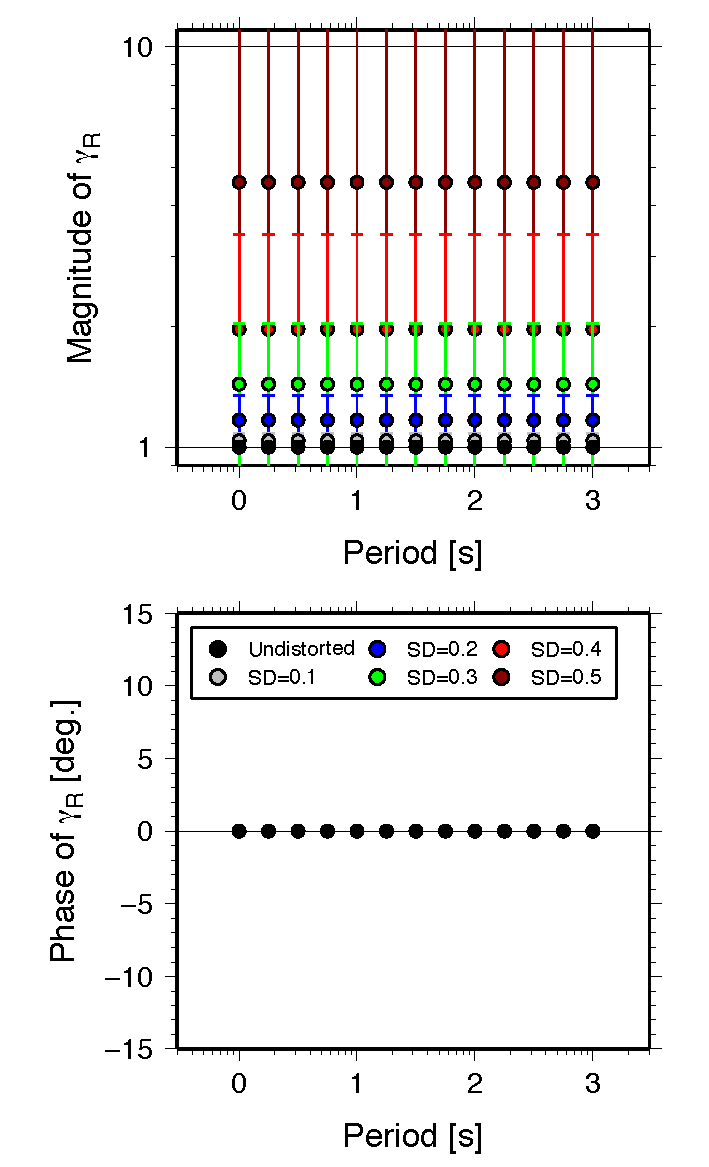
\includegraphics[scale=\plotmtrespscale]{\figdir/lyr11a_n25_d13a_distorted-sdxa_site_dispsd_gamma_magphs.pdf}
		\label{fig:gamma_regional_example_1d}
	}
	\subfigure[]{
		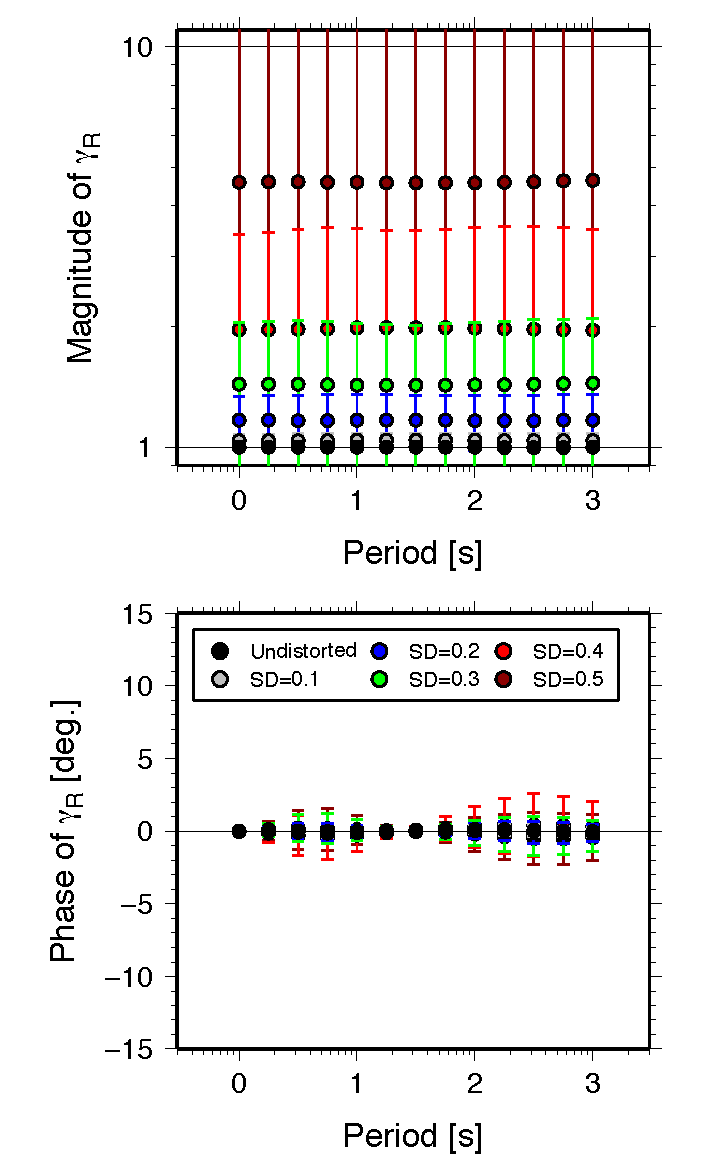
\includegraphics[scale=\plotmtrespscale]{\figdir/m02a-lyr11a_cb12-h0a2a-d05a-t01a_dr-e43n42_cb1X_loc-regi0_c-s40k-p0p0-pp1_d13a_distorted-sdxa_gamma_magphs.pdf}
		\label{fig:gamma_regional_example_3d}
	}
	\caption[Regional distortion indicators from 1D and 3D data distorted with different galvanic distortion strengths]{Regional distortion indicators from (a) 1D and (b) 3D examples with different galvanic distortion strengths.}
	\label{fig:gamma_regional_example}
\end{figure}

%% ==== Concluding paragraph: Local
From the synthetic examples, the local distortion indicator is able to determine the existence and strength of galvanic distortion, if contained in the data.
%
One of its possible and practical uses is to omit or decrease the constraints on the data from the stations that are heavily distorted (e.g., \texttt{syn01} and \texttt{syn02} in the example dataset), if the number of such stations is low.
%
When the number of heavily distorted stations is significant, the regional distortion indicator will be noticeable. The distortion removal or proper treatments, for example, the inversion simultaneously with galvanic distortion \citep[e.g.,][]{sasaki2006a, avdeeva2015a}, may be necessary.
%
However, if the magnitude of regional distortion indicator is rather small, i.e., the whole dataset is weakly distorted, such a complicated computation may be avoided.

%% ==== ====
\begin{comment}
\begin{itemize}
	\item \blue{Additional issues}
	\item \red{As shown in Fig. 25, the regional gamma becomes to be real-valued and frequency independent as a whole, even if local gamma at each site may be complex-valued
and frequency dependent. From this , we can decide whether the dataset is consistent with the assumed setting (regional structure well covered by the observation array + galvanic distorters).
If the regional 3D structure is not well covered, you will have complex-valued and frequency dependent regional gamma.}
\end{itemize}
\end{comment}



